% Options for packages loaded elsewhere
\PassOptionsToPackage{unicode}{hyperref}
\PassOptionsToPackage{hyphens}{url}
%
\documentclass[
  ignorenonframetext,
]{beamer}
\usepackage{pgfpages}
\setbeamertemplate{caption}[numbered]
\setbeamertemplate{caption label separator}{: }
\setbeamercolor{caption name}{fg=normal text.fg}
\beamertemplatenavigationsymbolsempty
% Prevent slide breaks in the middle of a paragraph
\widowpenalties 1 10000
\raggedbottom
\setbeamertemplate{part page}{
  \centering
  \begin{beamercolorbox}[sep=16pt,center]{part title}
    \usebeamerfont{part title}\insertpart\par
  \end{beamercolorbox}
}
\setbeamertemplate{section page}{
  \centering
  \begin{beamercolorbox}[sep=12pt,center]{part title}
    \usebeamerfont{section title}\insertsection\par
  \end{beamercolorbox}
}
\setbeamertemplate{subsection page}{
  \centering
  \begin{beamercolorbox}[sep=8pt,center]{part title}
    \usebeamerfont{subsection title}\insertsubsection\par
  \end{beamercolorbox}
}
\AtBeginPart{
  \frame{\partpage}
}
\AtBeginSection{
  \ifbibliography
  \else
    \frame{\sectionpage}
  \fi
}
\AtBeginSubsection{
  \frame{\subsectionpage}
}
\usepackage{amsmath,amssymb}
\usepackage{iftex}
\ifPDFTeX
  \usepackage[T1]{fontenc}
  \usepackage[utf8]{inputenc}
  \usepackage{textcomp} % provide euro and other symbols
\else % if luatex or xetex
  \usepackage{unicode-math} % this also loads fontspec
  \defaultfontfeatures{Scale=MatchLowercase}
  \defaultfontfeatures[\rmfamily]{Ligatures=TeX,Scale=1}
\fi
\usepackage{lmodern}
\usetheme[]{CambridgeUS}
\usecolortheme{seagull}
\usefonttheme{professionalfonts}
\ifPDFTeX\else
  % xetex/luatex font selection
\fi
% Use upquote if available, for straight quotes in verbatim environments
\IfFileExists{upquote.sty}{\usepackage{upquote}}{}
\IfFileExists{microtype.sty}{% use microtype if available
  \usepackage[]{microtype}
  \UseMicrotypeSet[protrusion]{basicmath} % disable protrusion for tt fonts
}{}
\makeatletter
\@ifundefined{KOMAClassName}{% if non-KOMA class
  \IfFileExists{parskip.sty}{%
    \usepackage{parskip}
  }{% else
    \setlength{\parindent}{0pt}
    \setlength{\parskip}{6pt plus 2pt minus 1pt}}
}{% if KOMA class
  \KOMAoptions{parskip=half}}
\makeatother
\usepackage{xcolor}
\newif\ifbibliography
\usepackage{color}
\usepackage{fancyvrb}
\newcommand{\VerbBar}{|}
\newcommand{\VERB}{\Verb[commandchars=\\\{\}]}
\DefineVerbatimEnvironment{Highlighting}{Verbatim}{commandchars=\\\{\}}
% Add ',fontsize=\small' for more characters per line
\usepackage{framed}
\definecolor{shadecolor}{RGB}{248,248,248}
\newenvironment{Shaded}{\begin{snugshade}}{\end{snugshade}}
\newcommand{\AlertTok}[1]{\textcolor[rgb]{0.94,0.16,0.16}{#1}}
\newcommand{\AnnotationTok}[1]{\textcolor[rgb]{0.56,0.35,0.01}{\textbf{\textit{#1}}}}
\newcommand{\AttributeTok}[1]{\textcolor[rgb]{0.13,0.29,0.53}{#1}}
\newcommand{\BaseNTok}[1]{\textcolor[rgb]{0.00,0.00,0.81}{#1}}
\newcommand{\BuiltInTok}[1]{#1}
\newcommand{\CharTok}[1]{\textcolor[rgb]{0.31,0.60,0.02}{#1}}
\newcommand{\CommentTok}[1]{\textcolor[rgb]{0.56,0.35,0.01}{\textit{#1}}}
\newcommand{\CommentVarTok}[1]{\textcolor[rgb]{0.56,0.35,0.01}{\textbf{\textit{#1}}}}
\newcommand{\ConstantTok}[1]{\textcolor[rgb]{0.56,0.35,0.01}{#1}}
\newcommand{\ControlFlowTok}[1]{\textcolor[rgb]{0.13,0.29,0.53}{\textbf{#1}}}
\newcommand{\DataTypeTok}[1]{\textcolor[rgb]{0.13,0.29,0.53}{#1}}
\newcommand{\DecValTok}[1]{\textcolor[rgb]{0.00,0.00,0.81}{#1}}
\newcommand{\DocumentationTok}[1]{\textcolor[rgb]{0.56,0.35,0.01}{\textbf{\textit{#1}}}}
\newcommand{\ErrorTok}[1]{\textcolor[rgb]{0.64,0.00,0.00}{\textbf{#1}}}
\newcommand{\ExtensionTok}[1]{#1}
\newcommand{\FloatTok}[1]{\textcolor[rgb]{0.00,0.00,0.81}{#1}}
\newcommand{\FunctionTok}[1]{\textcolor[rgb]{0.13,0.29,0.53}{\textbf{#1}}}
\newcommand{\ImportTok}[1]{#1}
\newcommand{\InformationTok}[1]{\textcolor[rgb]{0.56,0.35,0.01}{\textbf{\textit{#1}}}}
\newcommand{\KeywordTok}[1]{\textcolor[rgb]{0.13,0.29,0.53}{\textbf{#1}}}
\newcommand{\NormalTok}[1]{#1}
\newcommand{\OperatorTok}[1]{\textcolor[rgb]{0.81,0.36,0.00}{\textbf{#1}}}
\newcommand{\OtherTok}[1]{\textcolor[rgb]{0.56,0.35,0.01}{#1}}
\newcommand{\PreprocessorTok}[1]{\textcolor[rgb]{0.56,0.35,0.01}{\textit{#1}}}
\newcommand{\RegionMarkerTok}[1]{#1}
\newcommand{\SpecialCharTok}[1]{\textcolor[rgb]{0.81,0.36,0.00}{\textbf{#1}}}
\newcommand{\SpecialStringTok}[1]{\textcolor[rgb]{0.31,0.60,0.02}{#1}}
\newcommand{\StringTok}[1]{\textcolor[rgb]{0.31,0.60,0.02}{#1}}
\newcommand{\VariableTok}[1]{\textcolor[rgb]{0.00,0.00,0.00}{#1}}
\newcommand{\VerbatimStringTok}[1]{\textcolor[rgb]{0.31,0.60,0.02}{#1}}
\newcommand{\WarningTok}[1]{\textcolor[rgb]{0.56,0.35,0.01}{\textbf{\textit{#1}}}}
\setlength{\emergencystretch}{3em} % prevent overfull lines
\providecommand{\tightlist}{%
  \setlength{\itemsep}{0pt}\setlength{\parskip}{0pt}}
\setcounter{secnumdepth}{-\maxdimen} % remove section numbering
\usepackage{placeins}
\usepackage{color}
\usepackage{bm}
\usepackage{amsmath}
\usepackage{algorithm}
\usepackage[]{algpseudocode}
\usepackage{tabularx}
\usepackage{multirow}
\usepackage[most]{tcolorbox}
\usepackage{tikz}
\usepackage{lipsum}
\usepackage{mathtools}
\usepackage{actuarialangle}
\ifLuaTeX
  \usepackage{selnolig}  % disable illegal ligatures
\fi
\IfFileExists{bookmark.sty}{\usepackage{bookmark}}{\usepackage{hyperref}}
\IfFileExists{xurl.sty}{\usepackage{xurl}}{} % add URL line breaks if available
\urlstyle{same}
\hypersetup{
  pdftitle={MAT 3850 : Week 3},
  pdfauthor={Fall 2023},
  hidelinks,
  pdfcreator={LaTeX via pandoc}}

\title{MAT 3850 : Week 3}
\author{Fall 2023}
\date{}
\institute{App State}

\begin{document}
\frame{\titlepage}

\hypertarget{outline-for-the-week}{%
\section{Outline for the week}\label{outline-for-the-week}}

\begin{frame}{By the end of the week:}
\protect\hypertarget{by-the-end-of-the-week}{}
\begin{itemize}
\tightlist
\item
  Data Wrangling
\item
  ``Tidy'' data
\end{itemize}
\end{frame}

\hypertarget{data-wrangling}{%
\section{Data Wrangling}\label{data-wrangling}}

\begin{frame}[fragile]{Data Wrangling}
\protect\hypertarget{data-wrangling-1}{}
In this chapter, we'll introduce a series of functions from the
\texttt{dplyr} package for data wrangling

\begin{itemize}
\tightlist
\item
  We will be able to take a data frame and \textbf{``wrangle'' it
  (transform it)} to suit your needs. Such functions include:
\end{itemize}

\begin{enumerate}
\item
  \texttt{filter()} a data frame's existing rows to only pick out a
  subset of them.
\item
  \texttt{summarize()} one or more of its columns/variables with a
  summary statistic.
\item
  \texttt{group\_by()} its rows. In other words, assign different rows
  to be part of the same group.

  \begin{itemize}
  \tightlist
  \item
    We can then combine \texttt{group\_by(}) with \texttt{summarize()}
    to report summary statistics for each group separately.
  \end{itemize}
\end{enumerate}
\end{frame}

\begin{frame}[fragile]{Data Wrangling}
\protect\hypertarget{data-wrangling-2}{}
\begin{enumerate}
\setcounter{enumi}{3}
\item
  \texttt{mutate()} its existing columns/variables to create new ones.
  For example, convert hourly temperature recordings from degrees
  Fahrenheit to degrees Celsius.
\item
  \texttt{arrange()} its rows. For example, sort the rows of weather in
  ascending or descending order of temp.
\item
  \texttt{join()} it with another data frame by matching along a ``key''
  variable. In other words, merge these two data frames together.
\end{enumerate}

The further benefit to learning to use the \texttt{dplyr} package for
data wrangling is its its similarity to the \textbf{SQL} (database
querying language).
\end{frame}

\begin{frame}[fragile]{Needed packages}
\protect\hypertarget{needed-packages}{}
Let's load all the packages needed for this chapter. You need to install
them if you haven't already.

\small

\begin{Shaded}
\begin{Highlighting}[]
\FunctionTok{library}\NormalTok{(nycflights13)}
\FunctionTok{library}\NormalTok{(ggplot2)}
\FunctionTok{library}\NormalTok{(dplyr)}
\end{Highlighting}
\end{Shaded}

\normalsize
\end{frame}

\begin{frame}[fragile]{The pipe operator: \%\textgreater\%}
\protect\hypertarget{the-pipe-operator}{}
Before we start, let's first introduce a nifty tool that gets loaded
with the \texttt{dplyr} package: \textbf{the pipe operator
\%\textgreater\%}.

\begin{itemize}
\item
  The pipe operator allows us to combine multiple operations in R into a
  single sequential chain of actions.
\item
  Let's start with a hypothetical example:

  \begin{itemize}
  \tightlist
  \item
    Say you would like to perform a hypothetical sequence of operations
    on a hypothetical data frame \(x\)
  \item
    using hypothetical functions f(), g(), and h():
  \end{itemize}
\end{itemize}

\begin{enumerate}
\tightlist
\item
  Take \(x\) then
\item
  Use \(x\) as an input to a function \(f()\) then
\item
  Use the output of \(f(x)\) as an input to a function \(g()\) then
\item
  Use the output of \(g(f(x))\) as an input to a function \(h()\)
\end{enumerate}
\end{frame}

\begin{frame}[fragile]{The pipe operator: \%\textgreater\%}
\protect\hypertarget{the-pipe-operator-1}{}
One way to achieve this sequence of operations is by using nesting
parentheses as follows:

\small

\begin{Shaded}
\begin{Highlighting}[]
\FunctionTok{h}\NormalTok{(}\FunctionTok{g}\NormalTok{(}\FunctionTok{f}\NormalTok{(x)))}
\end{Highlighting}
\end{Shaded}

\normalsize

You can obtain the same output as the hypothetical sequence of functions
as follows:

\tiny

\begin{Shaded}
\begin{Highlighting}[]
\NormalTok{x}\SpecialCharTok{\%\textgreater{}\%}              \CommentTok{\# take x}
  \FunctionTok{f}\NormalTok{() }\SpecialCharTok{\%\textgreater{}\%}         \CommentTok{\# Use this output as the input to the next function f() then}
  \FunctionTok{g}\NormalTok{() }\SpecialCharTok{\%\textgreater{}\%}         \CommentTok{\# Use this output as the input to the next function g() then}
  \FunctionTok{h}\NormalTok{()             }\CommentTok{\# Use this output as the input to the next function h()}
\end{Highlighting}
\end{Shaded}

\normalsize

This is much more human-readable because you can clearly read the
sequence of operations line-by-line.
\end{frame}

\begin{frame}{The pipe operator: \%\textgreater\%}
\protect\hypertarget{the-pipe-operator-2}{}
\begin{center}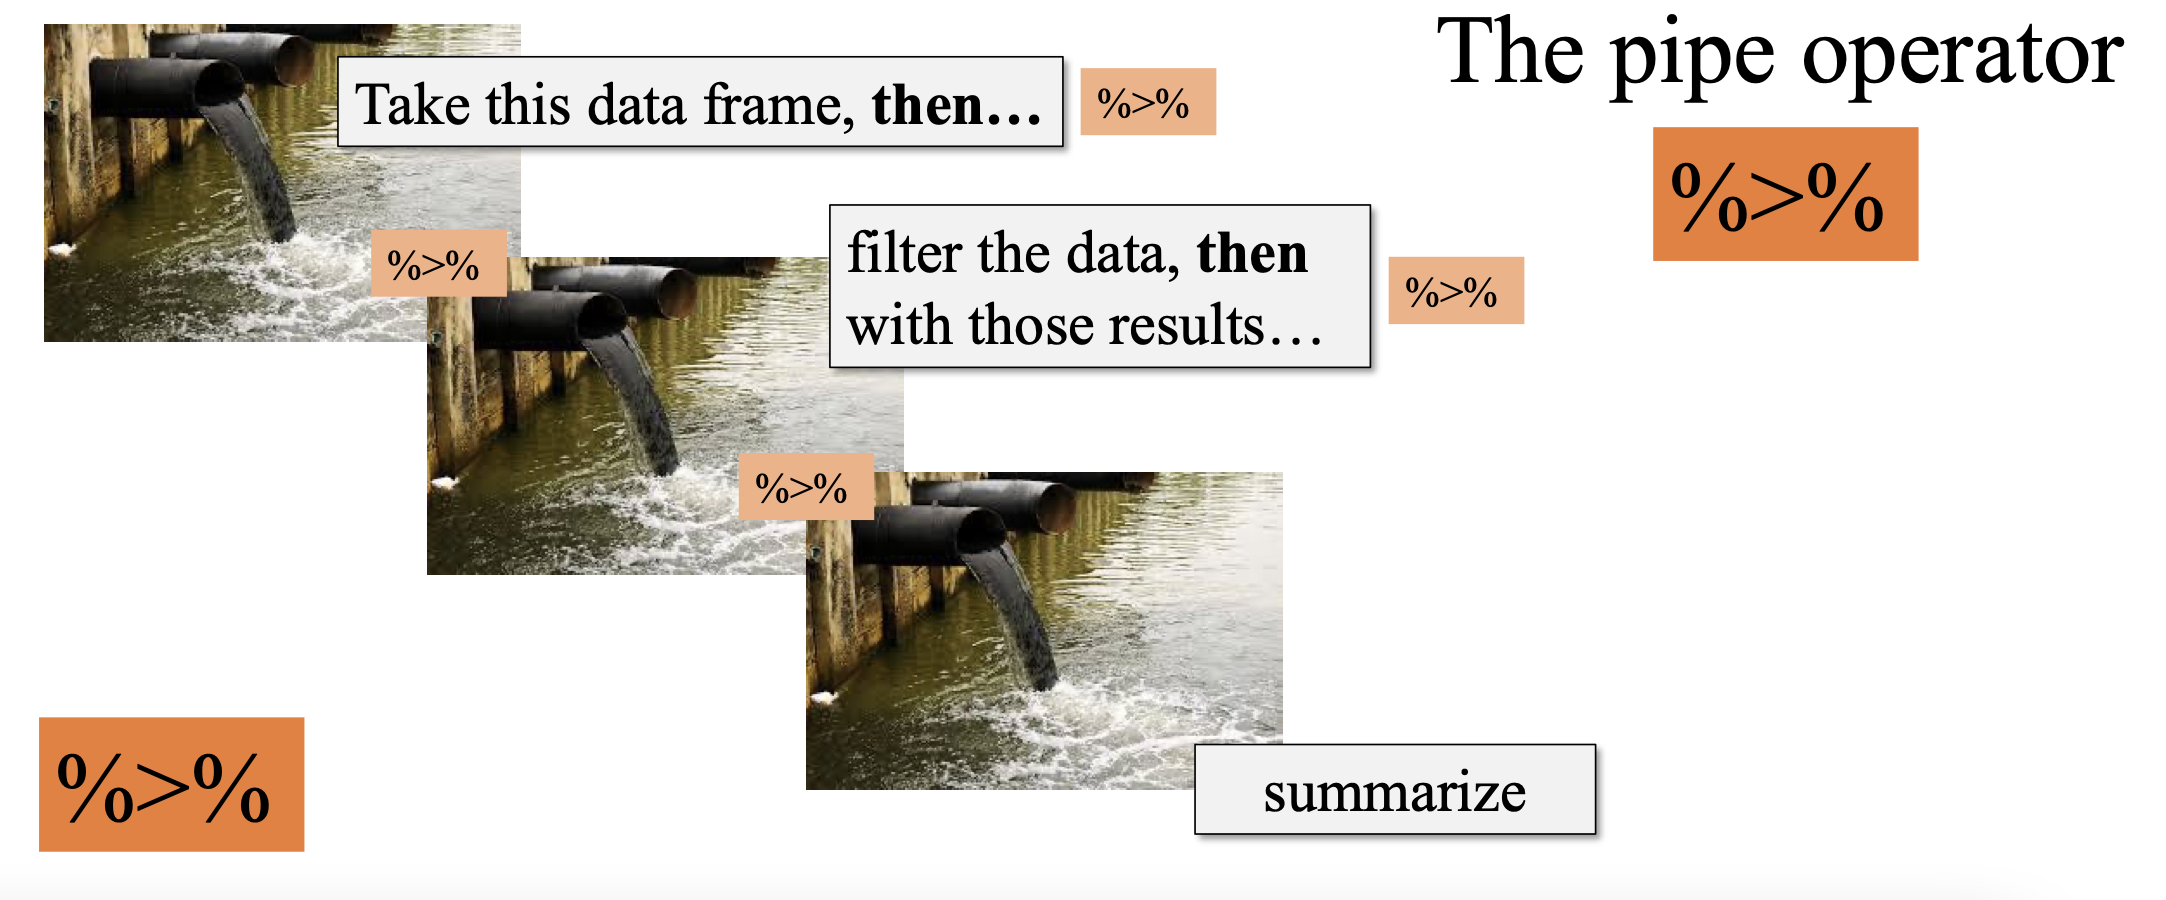
\includegraphics[width=0.8\linewidth,height=0.6\textheight]{week3_9} \end{center}
\end{frame}

\begin{frame}[fragile]{The pipe operator: \%\textgreater\%}
\protect\hypertarget{the-pipe-operator-3}{}
For example:

\small

\begin{Shaded}
\begin{Highlighting}[]
\NormalTok{alaska\_flights }\OtherTok{\textless{}{-}}\NormalTok{ flights }\SpecialCharTok{\%\textgreater{}\%} 
  \FunctionTok{filter}\NormalTok{(carrier }\SpecialCharTok{==} \StringTok{"AS"}\NormalTok{)}
\end{Highlighting}
\end{Shaded}

\normalsize

Note that the pipe operator \%\textgreater\% has to come at the end of
lines.
\end{frame}

\begin{frame}[fragile]{\texttt{filter} rows}
\protect\hypertarget{filter-rows}{}
\begin{center}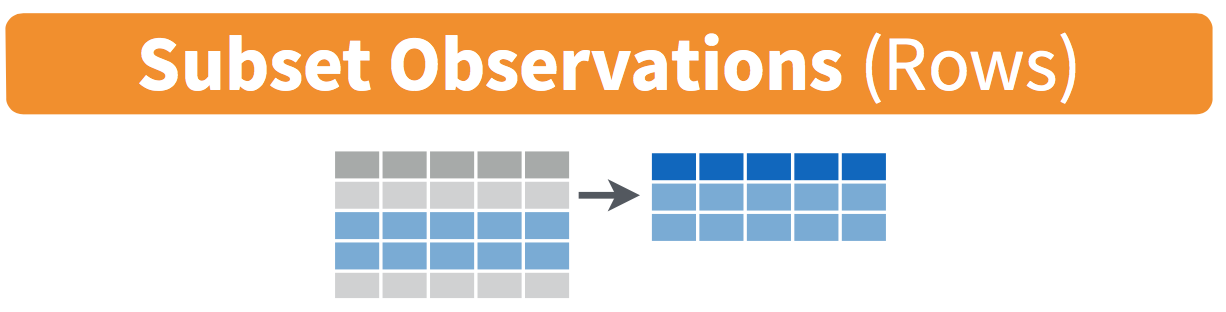
\includegraphics[width=0.7\linewidth,height=0.4\textheight]{week3_1} \end{center}

The \texttt{filter()} function allows you to specify criteria about the
values of a variable in your dataset and then filters out only the rows
that match that criteria.
\end{frame}

\begin{frame}[fragile]{\texttt{filter} rows}
\protect\hypertarget{filter-rows-1}{}
\begin{itemize}
\item
  We begin by focusing only on flights from New York City to Portland,
  Oregon.

  \begin{itemize}
  \tightlist
  \item
    The dest destination code (or airport code) for Portland, Oregon is
    ``PDX''.
  \item
    Run the following and look at the results in RStudio's spreadsheet
    viewer to ensure that only flights heading to Portland are chosen
    here:
  \end{itemize}
\end{itemize}

\small

\begin{Shaded}
\begin{Highlighting}[]
\NormalTok{portland\_flights }\OtherTok{\textless{}{-}}\NormalTok{ flights }\SpecialCharTok{\%\textgreater{}\%} 
  \FunctionTok{filter}\NormalTok{(dest }\SpecialCharTok{==} \StringTok{"PDX"}\NormalTok{)}
\CommentTok{\#View(portland\_flights)}
\end{Highlighting}
\end{Shaded}

\normalsize

We test for equality using the double equal sign \texttt{==} and not a
single equal sign \texttt{=}.
\end{frame}

\begin{frame}[fragile]{\texttt{filter} rows}
\protect\hypertarget{filter-rows-2}{}
\begin{itemize}
\item
  You can use other operators beyond just the \texttt{==} operator that
  tests for equality:

  \begin{itemize}
  \tightlist
  \item
    \texttt{\textgreater{}} corresponds to ``greater than''
  \item
    \texttt{\textless{}} corresponds to ``less than''
  \item
    \texttt{\textgreater{}=} corresponds to ``greater than or equal to''
  \item
    \texttt{\textless{}=} corresponds to ``less than or equal to''
  \item
    \texttt{!=} corresponds to ``not equal to.'' The ! is used in many
    programming languages to indicate ``not.''
  \end{itemize}
\item
  Furthermore, you can combine multiple criteria using operators that
  make comparisons:

  \begin{itemize}
  \tightlist
  \item
    \texttt{\textbar{}} corresponds to ``or''
  \item
    \texttt{\&} corresponds to ``and''
  \end{itemize}
\end{itemize}
\end{frame}

\begin{frame}[fragile]{\texttt{filter} rows}
\protect\hypertarget{filter-rows-3}{}
\begin{itemize}
\item
  We filter flights for all rows that

  \begin{itemize}
  \tightlist
  \item
    departed from JFK and
  \item
    were heading to Burlington, Vermont (``BTV'') or Seattle, Washington
    (``SEA'') and
  \item
    departed in the months of October, November, or December.
  \end{itemize}
\end{itemize}

\tiny

\begin{Shaded}
\begin{Highlighting}[]
\NormalTok{btv\_sea\_flights\_fall }\OtherTok{\textless{}{-}}\NormalTok{ flights }\SpecialCharTok{\%\textgreater{}\%} 
  \FunctionTok{filter}\NormalTok{(origin }\SpecialCharTok{==} \StringTok{"JFK"} \SpecialCharTok{\&}\NormalTok{ (dest }\SpecialCharTok{==} \StringTok{"BTV"} \SpecialCharTok{|}\NormalTok{ dest }\SpecialCharTok{==} \StringTok{"SEA"}\NormalTok{) }\SpecialCharTok{\&}\NormalTok{ month }\SpecialCharTok{\textgreater{}=} \DecValTok{10}\NormalTok{)}
\CommentTok{\#View(btv\_sea\_flights\_fall)}
\end{Highlighting}
\end{Shaded}

\normalsize

We can often skip the use of \& and just separate our conditions with a
comma

\tiny

\begin{Shaded}
\begin{Highlighting}[]
\NormalTok{btv\_sea\_flights\_fall }\OtherTok{\textless{}{-}}\NormalTok{ flights }\SpecialCharTok{\%\textgreater{}\%} 
  \FunctionTok{filter}\NormalTok{(origin }\SpecialCharTok{==} \StringTok{"JFK"}\NormalTok{, (dest }\SpecialCharTok{==} \StringTok{"BTV"} \SpecialCharTok{|}\NormalTok{ dest }\SpecialCharTok{==} \StringTok{"SEA"}\NormalTok{), month }\SpecialCharTok{\textgreater{}=} \DecValTok{10}\NormalTok{)}
\CommentTok{\#View(btv\_sea\_flights\_fall)}
\end{Highlighting}
\end{Shaded}

\normalsize
\end{frame}

\begin{frame}[fragile]{\texttt{filter} rows}
\protect\hypertarget{filter-rows-4}{}
Lets filter rows corresponding to flights that didn't go to Burlington,
VT or Seattle, WA.

\tiny

\begin{Shaded}
\begin{Highlighting}[]
\NormalTok{not\_BTV\_SEA }\OtherTok{\textless{}{-}}\NormalTok{ flights }\SpecialCharTok{\%\textgreater{}\%} 
  \FunctionTok{filter}\NormalTok{(}\SpecialCharTok{!}\NormalTok{(dest }\SpecialCharTok{==} \StringTok{"BTV"} \SpecialCharTok{|}\NormalTok{ dest }\SpecialCharTok{==} \StringTok{"SEA"}\NormalTok{))}
\CommentTok{\#View(not\_BTV\_SEA)}
\end{Highlighting}
\end{Shaded}

\normalsize

Note note the careful use of parentheses. The code below will produce
different results. \tiny

\begin{Shaded}
\begin{Highlighting}[]
\NormalTok{flights }\SpecialCharTok{\%\textgreater{}\%} \FunctionTok{filter}\NormalTok{(}\SpecialCharTok{!}\NormalTok{dest }\SpecialCharTok{==} \StringTok{"BTV"} \SpecialCharTok{|}\NormalTok{ dest }\SpecialCharTok{==} \StringTok{"SEA"}\NormalTok{)}
\end{Highlighting}
\end{Shaded}

\normalsize
\end{frame}

\begin{frame}[fragile]{\texttt{filter} rows}
\protect\hypertarget{filter-rows-5}{}
Say we have a larger number of airports we want to filter for. We could
continue to use the \texttt{\textbar{}} (or) operator:

\tiny

\begin{Shaded}
\begin{Highlighting}[]
\NormalTok{many\_airports }\OtherTok{\textless{}{-}}\NormalTok{ flights }\SpecialCharTok{\%\textgreater{}\%} 
  \FunctionTok{filter}\NormalTok{(dest }\SpecialCharTok{==} \StringTok{"SEA"} \SpecialCharTok{|}\NormalTok{ dest }\SpecialCharTok{==} \StringTok{"SFO"} \SpecialCharTok{|}\NormalTok{ dest }\SpecialCharTok{==} \StringTok{"PDX"} \SpecialCharTok{|} 
\NormalTok{         dest }\SpecialCharTok{==} \StringTok{"BTV"} \SpecialCharTok{|}\NormalTok{ dest }\SpecialCharTok{==} \StringTok{"BDL"}\NormalTok{)}
\end{Highlighting}
\end{Shaded}

\normalsize

A shorter approach will be to use \texttt{\%in\%} operator along with
the \texttt{c()} function.

\tiny

\begin{Shaded}
\begin{Highlighting}[]
\NormalTok{many\_airports }\OtherTok{\textless{}{-}}\NormalTok{ flights }\SpecialCharTok{\%\textgreater{}\%} 
  \FunctionTok{filter}\NormalTok{(dest }\SpecialCharTok{\%in\%} \FunctionTok{c}\NormalTok{(}\StringTok{"SEA"}\NormalTok{, }\StringTok{"SFO"}\NormalTok{, }\StringTok{"PDX"}\NormalTok{, }\StringTok{"BTV"}\NormalTok{, }\StringTok{"BDL"}\NormalTok{))}
\CommentTok{\#View(many\_airports)}
\end{Highlighting}
\end{Shaded}

\normalsize

The \texttt{\%in\%} operator is useful for looking for matches commonly
in one vector/variable compared to another.
\end{frame}

\begin{frame}{\texttt{summarize} variables}
\protect\hypertarget{summarize-variables}{}
The next common task when working with data frames is to compute
\textbf{summary statistics}. Summary statistics are single numerical
values that summarize a large number of values.

\begin{itemize}
\item
  Commonly known examples of summary statistics include

  \begin{itemize}
  \tightlist
  \item
    the mean (also called the average) ,
  \item
    the median (the middle value),
  \item
    the sum,
  \item
    the smallest value also called the minimum,
  \item
    the largest value also called the maximum, and
  \item
    the standard deviation.
  \end{itemize}
\end{itemize}

\begin{center}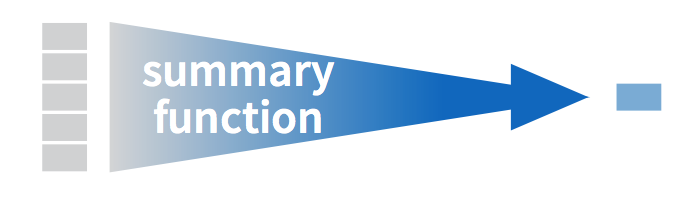
\includegraphics[width=0.6\linewidth,height=0.2\textheight]{week3_2} \end{center}
\end{frame}

\begin{frame}[fragile]{\texttt{summarize} variables}
\protect\hypertarget{summarize-variables-1}{}
Let's calculate two summary statistics (mean and standard deviation) of
the \texttt{temp} temperature variable in the \texttt{weather} data
frame from \texttt{nycflights13} package.

\small

\begin{Shaded}
\begin{Highlighting}[]
\NormalTok{summary\_temp }\OtherTok{\textless{}{-}}\NormalTok{ weather }\SpecialCharTok{\%\textgreater{}\%} 
  \FunctionTok{summarize}\NormalTok{(}\AttributeTok{mean =} \FunctionTok{mean}\NormalTok{(temp), }\AttributeTok{std\_dev =} \FunctionTok{sd}\NormalTok{(temp))}
\NormalTok{summary\_temp}
\end{Highlighting}
\end{Shaded}

\begin{verbatim}
## # A tibble: 1 x 2
##    mean std_dev
##   <dbl>   <dbl>
## 1    NA      NA
\end{verbatim}

\normalsize

\texttt{NA} values returned because there are missing values in the
\texttt{temp} data.
\end{frame}

\begin{frame}[fragile]{\texttt{summarize} variables}
\protect\hypertarget{summarize-variables-2}{}
\begin{itemize}
\item
  To work around this fact:

  \begin{itemize}
  \tightlist
  \item
    you can set the \texttt{na.rm} argument to TRUE,
  \item
    where \texttt{rm} is short for ``remove''; this will ignore any NA
    missing values and only return the summary value for all non-missing
    values.
  \end{itemize}
\end{itemize}

\small

\begin{Shaded}
\begin{Highlighting}[]
\NormalTok{summary\_temp }\OtherTok{\textless{}{-}}\NormalTok{ weather }\SpecialCharTok{\%\textgreater{}\%} 
  \FunctionTok{summarize}\NormalTok{(}\AttributeTok{mean =} \FunctionTok{mean}\NormalTok{(temp, }\AttributeTok{na.rm =} \ConstantTok{TRUE}\NormalTok{), }
            \AttributeTok{std\_dev =} \FunctionTok{sd}\NormalTok{(temp, }\AttributeTok{na.rm =} \ConstantTok{TRUE}\NormalTok{))}
\NormalTok{summary\_temp}
\end{Highlighting}
\end{Shaded}

\begin{verbatim}
## # A tibble: 1 x 2
##    mean std_dev
##   <dbl>   <dbl>
## 1  55.3    17.8
\end{verbatim}

\normalsize
\end{frame}

\begin{frame}[fragile]{\texttt{summarize} variables}
\protect\hypertarget{summarize-variables-3}{}
Other summary functions we can use inside the \texttt{summarize()}:

\begin{itemize}
\tightlist
\item
  \texttt{mean()}: the average
\item
  \texttt{sd()}: the standard deviation, which is a measure of spread
\item
  \texttt{min()} and \texttt{max()}: the minimum and maximum values,
  respectively
\item
  \texttt{IQR()}: interquartile range
\item
  \texttt{sum()}: the total amount when adding multiple numbers
\item
  \texttt{n()}: a count of the number of rows in each group. This
  particular summary function will make more sense when
  \texttt{group\_by()}.
\end{itemize}
\end{frame}

\begin{frame}{\texttt{group\_by} rows}
\protect\hypertarget{group_by-rows}{}
\begin{itemize}
\item
  Say instead of a single mean temperature for the whole year, you would
  like 12 mean temperatures, one for each of the 12 months separately.

  \begin{itemize}
  \tightlist
  \item
    We would like to compute the mean temperature split by month.
  \item
    We can do this by ``grouping'' temperature observations by the
    values of another variable, in this case by the 12 values of the
    variable month.
  \end{itemize}
\end{itemize}

\begin{center}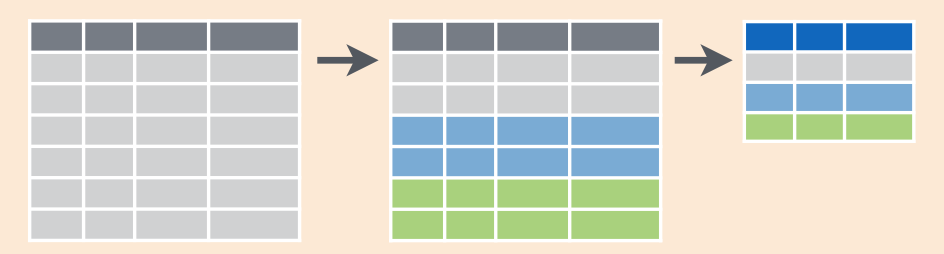
\includegraphics[width=0.8\linewidth,height=0.4\textheight]{week3_3} \end{center}
\end{frame}

\begin{frame}[fragile]{\texttt{group\_by} rows}
\protect\hypertarget{group_by-rows-1}{}
\tiny

\begin{Shaded}
\begin{Highlighting}[]
\NormalTok{summary\_monthly\_temp }\OtherTok{\textless{}{-}}\NormalTok{ weather }\SpecialCharTok{\%\textgreater{}\%} 
  \FunctionTok{group\_by}\NormalTok{(month) }\SpecialCharTok{\%\textgreater{}\%} 
  \FunctionTok{summarize}\NormalTok{(}\AttributeTok{mean =} \FunctionTok{mean}\NormalTok{(temp, }\AttributeTok{na.rm =} \ConstantTok{TRUE}\NormalTok{), }
            \AttributeTok{std\_dev =} \FunctionTok{sd}\NormalTok{(temp, }\AttributeTok{na.rm =} \ConstantTok{TRUE}\NormalTok{),}
            \AttributeTok{count =} \FunctionTok{n}\NormalTok{())}
\NormalTok{summary\_monthly\_temp}
\end{Highlighting}
\end{Shaded}

\begin{verbatim}
## # A tibble: 12 x 4
##    month  mean std_dev count
##    <int> <dbl>   <dbl> <int>
##  1     1  35.6   10.2   2226
##  2     2  34.3    6.98  2010
##  3     3  39.9    6.25  2227
##  4     4  51.7    8.79  2159
##  5     5  61.8    9.68  2232
##  6     6  72.2    7.55  2160
##  7     7  80.1    7.12  2228
##  8     8  74.5    5.19  2217
##  9     9  67.4    8.47  2159
## 10    10  60.1    8.85  2212
## 11    11  45.0   10.4   2141
## 12    12  38.4    9.98  2144
\end{verbatim}

\normalsize
\end{frame}

\begin{frame}[fragile]{Grouping by more than one variable}
\protect\hypertarget{grouping-by-more-than-one-variable}{}
We can also group by more than one variable

\tiny

\begin{Shaded}
\begin{Highlighting}[]
\NormalTok{by\_origin\_monthly }\OtherTok{\textless{}{-}}\NormalTok{ flights }\SpecialCharTok{\%\textgreater{}\%} 
  \FunctionTok{group\_by}\NormalTok{(origin, month) }\SpecialCharTok{\%\textgreater{}\%} 
  \FunctionTok{summarize}\NormalTok{(}\AttributeTok{count =} \FunctionTok{n}\NormalTok{())}
\NormalTok{by\_origin\_monthly}
\end{Highlighting}
\end{Shaded}

\begin{verbatim}
## # A tibble: 36 x 3
## # Groups:   origin [3]
##    origin month count
##    <chr>  <int> <int>
##  1 EWR        1  9893
##  2 EWR        2  9107
##  3 EWR        3 10420
##  4 EWR        4 10531
##  5 EWR        5 10592
##  6 EWR        6 10175
##  7 EWR        7 10475
##  8 EWR        8 10359
##  9 EWR        9  9550
## 10 EWR       10 10104
## # i 26 more rows
\end{verbatim}

\normalsize

Observe that there are 36 rows to \texttt{by\_origin\_monthly} because
there are 12 months for 3 airports (\texttt{EWR}, \texttt{JFK}, and
\texttt{LGA}).
\end{frame}

\begin{frame}[fragile]{Grouping by more than one variable}
\protect\hypertarget{grouping-by-more-than-one-variable-1}{}
Why do we \texttt{group\_by(origin,\ month)} and not
\texttt{group\_by(origin)} and then \texttt{group\_by(month)}? Let's
investigate:

\tiny

\begin{Shaded}
\begin{Highlighting}[]
\NormalTok{by\_origin\_monthly\_incorrect }\OtherTok{\textless{}{-}}\NormalTok{ flights }\SpecialCharTok{\%\textgreater{}\%} 
  \FunctionTok{group\_by}\NormalTok{(origin) }\SpecialCharTok{\%\textgreater{}\%} 
  \FunctionTok{group\_by}\NormalTok{(month) }\SpecialCharTok{\%\textgreater{}\%} 
  \FunctionTok{summarize}\NormalTok{(}\AttributeTok{count =} \FunctionTok{n}\NormalTok{())}
\NormalTok{by\_origin\_monthly\_incorrect}
\end{Highlighting}
\end{Shaded}

\begin{verbatim}
## # A tibble: 12 x 2
##    month count
##    <int> <int>
##  1     1 27004
##  2     2 24951
##  3     3 28834
##  4     4 28330
##  5     5 28796
##  6     6 28243
##  7     7 29425
##  8     8 29327
##  9     9 27574
## 10    10 28889
## 11    11 27268
## 12    12 28135
\end{verbatim}

\normalsize

The second \texttt{group\_by(month)} overwrote
\texttt{group\_by(origin)}.
\end{frame}

\begin{frame}{\texttt{mutate} existing variables}
\protect\hypertarget{mutate-existing-variables}{}
Another common transformation of data is to create/compute new variables
based on existing ones.

\begin{center}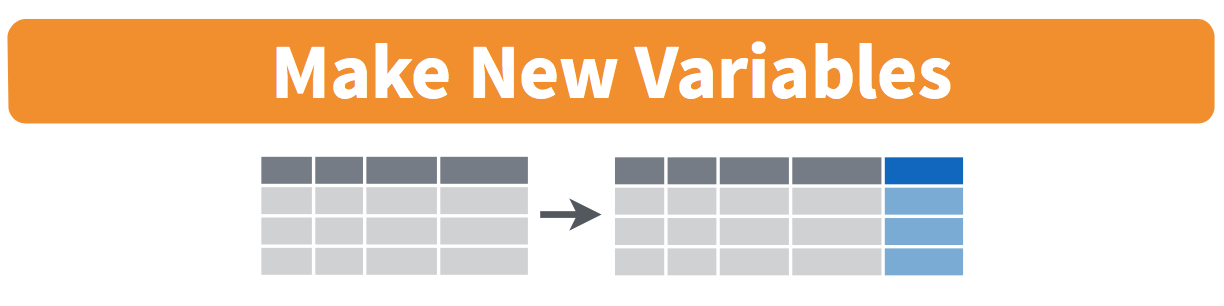
\includegraphics[width=0.8\linewidth,height=0.4\textheight]{week3_4} \end{center}

For example, we can create a new variable by converting temperatures
from \(^\circ\)F to \(^\circ\)C using the formula
\[\text{temp in C}=\frac{\text{temp in F}-32}{1.8}\]
\end{frame}

\begin{frame}[fragile]{\texttt{mutate} existing variables}
\protect\hypertarget{mutate-existing-variables-1}{}
We can apply this formula to the \texttt{temp} variable using the
\texttt{mutate()} function from the \texttt{dplyr} package.

\tiny

\begin{Shaded}
\begin{Highlighting}[]
\NormalTok{weather }\OtherTok{\textless{}{-}}\NormalTok{ weather }\SpecialCharTok{\%\textgreater{}\%} 
  \FunctionTok{mutate}\NormalTok{(}\AttributeTok{temp\_in\_C =}\NormalTok{ (temp }\SpecialCharTok{{-}} \DecValTok{32}\NormalTok{) }\SpecialCharTok{/} \FloatTok{1.8}\NormalTok{)}
\end{Highlighting}
\end{Shaded}

\normalsize

\begin{itemize}
\item
  In this code:

  \begin{itemize}
  \tightlist
  \item
    we \texttt{mutate()} the \texttt{weather} data frame by creating a
    new variable \texttt{temp\_in\_C\ =\ (temp\ -\ 32)\ /\ 1.8} and
  \item
    then overwrite the original weather data frame.
  \end{itemize}
\end{itemize}
\end{frame}

\begin{frame}[fragile]{\texttt{mutate} existing variables}
\protect\hypertarget{mutate-existing-variables-2}{}
Let's now compute monthly average temperatures in both \(^\circ\)F and
\(^\circ\)C.

\tiny

\begin{Shaded}
\begin{Highlighting}[]
\NormalTok{summary\_monthly\_temp }\OtherTok{\textless{}{-}}\NormalTok{ weather }\SpecialCharTok{\%\textgreater{}\%} 
  \FunctionTok{group\_by}\NormalTok{(month) }\SpecialCharTok{\%\textgreater{}\%} 
  \FunctionTok{summarize}\NormalTok{(}\AttributeTok{mean\_temp\_in\_F =} \FunctionTok{mean}\NormalTok{(temp, }\AttributeTok{na.rm =} \ConstantTok{TRUE}\NormalTok{), }
            \AttributeTok{mean\_temp\_in\_C =} \FunctionTok{mean}\NormalTok{(temp\_in\_C, }\AttributeTok{na.rm =} \ConstantTok{TRUE}\NormalTok{))}
\NormalTok{summary\_monthly\_temp}
\end{Highlighting}
\end{Shaded}

\begin{verbatim}
## # A tibble: 12 x 3
##    month mean_temp_in_F mean_temp_in_C
##    <int>          <dbl>          <dbl>
##  1     1           35.6           2.02
##  2     2           34.3           1.26
##  3     3           39.9           4.38
##  4     4           51.7          11.0 
##  5     5           61.8          16.6 
##  6     6           72.2          22.3 
##  7     7           80.1          26.7 
##  8     8           74.5          23.6 
##  9     9           67.4          19.7 
## 10    10           60.1          15.6 
## 11    11           45.0           7.22
## 12    12           38.4           3.58
\end{verbatim}

\normalsize
\end{frame}

\begin{frame}[fragile]{\texttt{mutate} existing variables}
\protect\hypertarget{mutate-existing-variables-3}{}
Let's consider another example.

\begin{itemize}
\item
  Passengers are often frustrated when their flight departs late, but
  aren't as annoyed if, in the end, pilots can make up some time during
  the flight.
\item
  This is known in the airline industry as \texttt{gain}, and we will
  create this variable using the \texttt{mutate()} function:
\end{itemize}

\tiny

\begin{Shaded}
\begin{Highlighting}[]
\NormalTok{flights }\OtherTok{\textless{}{-}}\NormalTok{ flights }\SpecialCharTok{\%\textgreater{}\%} 
  \FunctionTok{mutate}\NormalTok{(}\AttributeTok{gain =}\NormalTok{ dep\_delay }\SpecialCharTok{{-}}\NormalTok{ arr\_delay)}
\NormalTok{flights  }\SpecialCharTok{\%\textgreater{}\%} \FunctionTok{select}\NormalTok{(dep\_delay, arr\_delay, gain)}\SpecialCharTok{\%\textgreater{}\%} \FunctionTok{head}\NormalTok{()}
\end{Highlighting}
\end{Shaded}

\begin{verbatim}
## # A tibble: 6 x 3
##   dep_delay arr_delay  gain
##       <dbl>     <dbl> <dbl>
## 1         2        11    -9
## 2         4        20   -16
## 3         2        33   -31
## 4        -1       -18    17
## 5        -6       -25    19
## 6        -4        12   -16
\end{verbatim}

\normalsize
\end{frame}

\begin{frame}[fragile]{\texttt{mutate} existing variables}
\protect\hypertarget{mutate-existing-variables-4}{}
Let's look at some summary statistics of the \texttt{gain} variable

\tiny

\begin{Shaded}
\begin{Highlighting}[]
\NormalTok{gain\_summary }\OtherTok{\textless{}{-}}\NormalTok{ flights }\SpecialCharTok{\%\textgreater{}\%} 
  \FunctionTok{summarize}\NormalTok{(}
    \AttributeTok{min =} \FunctionTok{min}\NormalTok{(gain, }\AttributeTok{na.rm =} \ConstantTok{TRUE}\NormalTok{),}
    \AttributeTok{q1 =} \FunctionTok{quantile}\NormalTok{(gain, }\FloatTok{0.25}\NormalTok{, }\AttributeTok{na.rm =} \ConstantTok{TRUE}\NormalTok{),}
    \AttributeTok{median =} \FunctionTok{quantile}\NormalTok{(gain, }\FloatTok{0.5}\NormalTok{, }\AttributeTok{na.rm =} \ConstantTok{TRUE}\NormalTok{),}
    \AttributeTok{q3 =} \FunctionTok{quantile}\NormalTok{(gain, }\FloatTok{0.75}\NormalTok{, }\AttributeTok{na.rm =} \ConstantTok{TRUE}\NormalTok{),}
    \AttributeTok{max =} \FunctionTok{max}\NormalTok{(gain, }\AttributeTok{na.rm =} \ConstantTok{TRUE}\NormalTok{),}
    \AttributeTok{mean =} \FunctionTok{mean}\NormalTok{(gain, }\AttributeTok{na.rm =} \ConstantTok{TRUE}\NormalTok{),}
    \AttributeTok{sd =} \FunctionTok{sd}\NormalTok{(gain, }\AttributeTok{na.rm =} \ConstantTok{TRUE}\NormalTok{),}
    \AttributeTok{missing =} \FunctionTok{sum}\NormalTok{(}\FunctionTok{is.na}\NormalTok{(gain))}
\NormalTok{  )}
\NormalTok{gain\_summary}
\end{Highlighting}
\end{Shaded}

\begin{verbatim}
## # A tibble: 1 x 8
##     min    q1 median    q3   max  mean    sd missing
##   <dbl> <dbl>  <dbl> <dbl> <dbl> <dbl> <dbl>   <int>
## 1  -196    -3      7    17   109  5.66  18.0    9430
\end{verbatim}

\normalsize
\end{frame}

\begin{frame}[fragile]{\texttt{mutate} existing variables}
\protect\hypertarget{mutate-existing-variables-5}{}
Since \texttt{gain} is a numerical variable, we can visualize its
distribution using a histogram.

\tiny

\begin{Shaded}
\begin{Highlighting}[]
\FunctionTok{ggplot}\NormalTok{(}\AttributeTok{data =}\NormalTok{ flights, }\AttributeTok{mapping =} \FunctionTok{aes}\NormalTok{(}\AttributeTok{x =}\NormalTok{ gain)) }\SpecialCharTok{+}
  \FunctionTok{geom\_histogram}\NormalTok{(}\AttributeTok{color =} \StringTok{"white"}\NormalTok{, }\AttributeTok{bins =} \DecValTok{20}\NormalTok{)}
\end{Highlighting}
\end{Shaded}

\begin{center}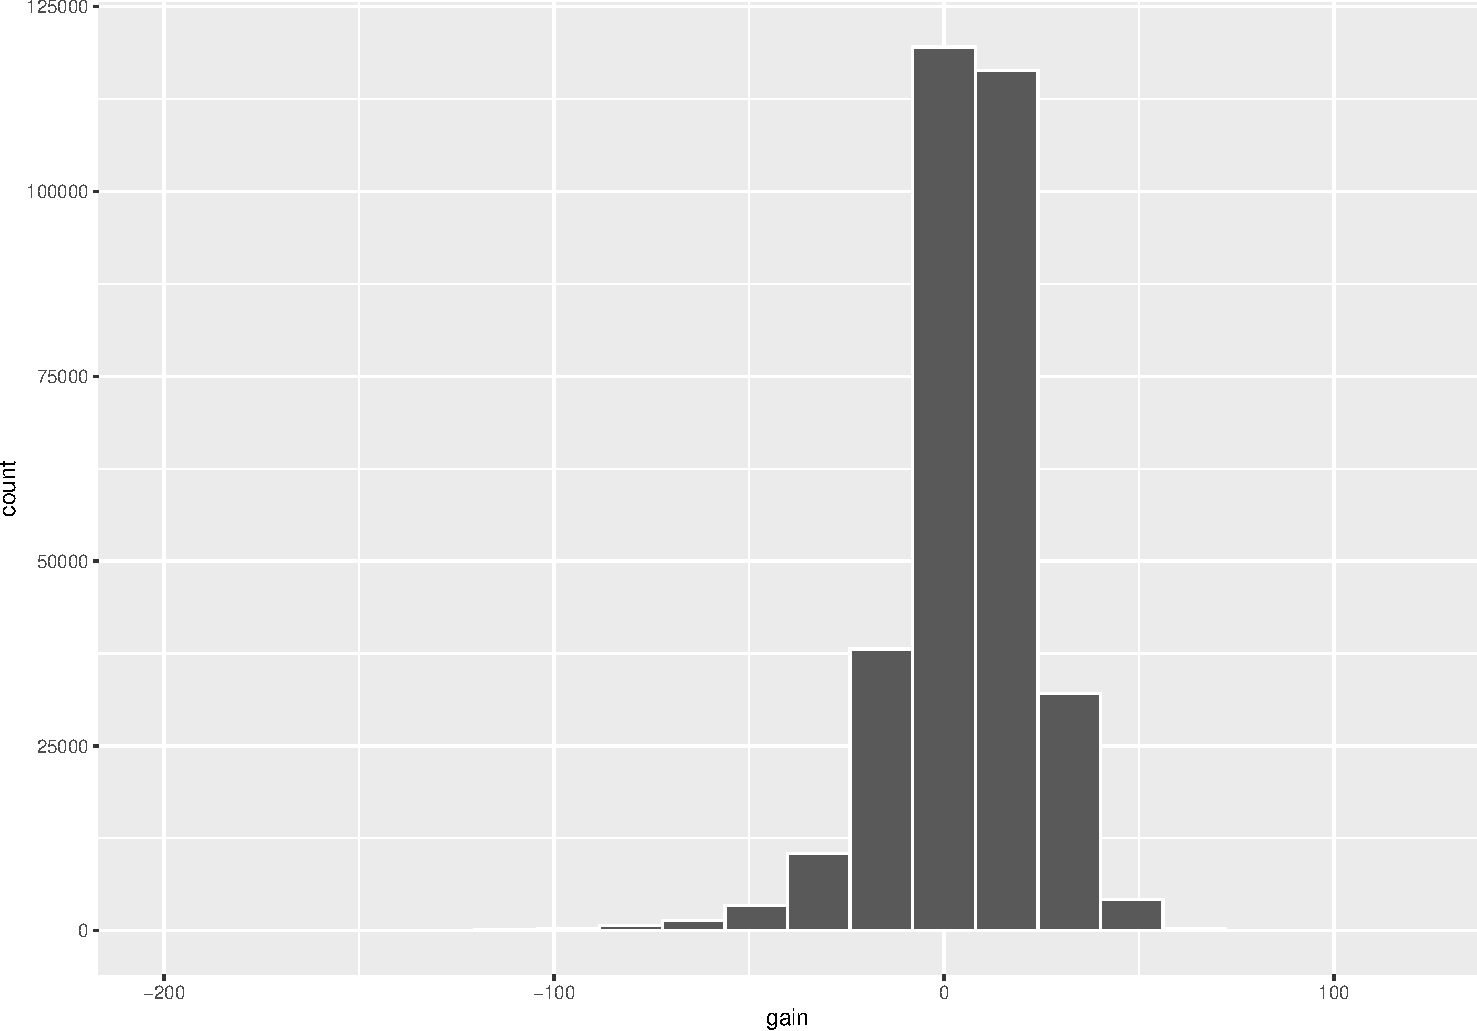
\includegraphics[width=0.7\linewidth,height=0.5\textheight]{Week3_files/figure-beamer/unnamed-chunk-26-1} \end{center}
\normalsize
\end{frame}

\begin{frame}[fragile]{\texttt{arrange} and sort rows}
\protect\hypertarget{arrange-and-sort-rows}{}
\begin{itemize}
\item
  One of the most commonly performed data wrangling tasks is to sort a
  data frame's rows in the alphanumeric order of one of the variables.
\item
  The \texttt{dplyr} package's \texttt{arrange()} function allows us to
  sort/reorder a data frame's rows according to the values of the
  specified variable.
\end{itemize}
\end{frame}

\begin{frame}[fragile]{\texttt{arrange} and sort rows}
\protect\hypertarget{arrange-and-sort-rows-1}{}
Suppose we are interested in determining the most frequent destination
airports for all domestic flights departing from New York City in 2013.

\tiny

\begin{Shaded}
\begin{Highlighting}[]
\NormalTok{freq\_dest }\OtherTok{\textless{}{-}}\NormalTok{ flights }\SpecialCharTok{\%\textgreater{}\%} 
  \FunctionTok{group\_by}\NormalTok{(dest) }\SpecialCharTok{\%\textgreater{}\%} 
  \FunctionTok{summarize}\NormalTok{(}\AttributeTok{num\_flights =} \FunctionTok{n}\NormalTok{())}
\NormalTok{freq\_dest}
\end{Highlighting}
\end{Shaded}

\begin{verbatim}
## # A tibble: 105 x 2
##    dest  num_flights
##    <chr>       <int>
##  1 ABQ           254
##  2 ACK           265
##  3 ALB           439
##  4 ANC             8
##  5 ATL         17215
##  6 AUS          2439
##  7 AVL           275
##  8 BDL           443
##  9 BGR           375
## 10 BHM           297
## # i 95 more rows
\end{verbatim}

\normalsize

Observe that by default the rows of the resulting \texttt{freq\_dest}
data frame are sorted in alphabetical order of destination.
\end{frame}

\begin{frame}[fragile]{\texttt{arrange} and sort rows}
\protect\hypertarget{arrange-and-sort-rows-2}{}
Say instead we would like to see the same data, but sorted from the most
to the least number of flights (\texttt{num\_flights}) instead

\tiny

\begin{Shaded}
\begin{Highlighting}[]
\NormalTok{freq\_dest }\SpecialCharTok{\%\textgreater{}\%} 
  \FunctionTok{arrange}\NormalTok{(num\_flights)}
\end{Highlighting}
\end{Shaded}

\begin{verbatim}
## # A tibble: 105 x 2
##    dest  num_flights
##    <chr>       <int>
##  1 LEX             1
##  2 LGA             1
##  3 ANC             8
##  4 SBN            10
##  5 HDN            15
##  6 MTJ            15
##  7 EYW            17
##  8 PSP            19
##  9 JAC            25
## 10 BZN            36
## # i 95 more rows
\end{verbatim}

\normalsize

This is, however, the opposite of what we want. The rows are sorted with
the least frequent destination airports displayed first.
\end{frame}

\begin{frame}[fragile]{\texttt{arrange} and sort rows}
\protect\hypertarget{arrange-and-sort-rows-3}{}
To switch the ordering to be in ``descending'' order instead, we use the
\texttt{desc()} function as so:

\tiny

\begin{Shaded}
\begin{Highlighting}[]
\NormalTok{freq\_dest }\SpecialCharTok{\%\textgreater{}\%} 
  \FunctionTok{arrange}\NormalTok{(}\FunctionTok{desc}\NormalTok{(num\_flights))}
\end{Highlighting}
\end{Shaded}

\begin{verbatim}
## # A tibble: 105 x 2
##    dest  num_flights
##    <chr>       <int>
##  1 ORD         17283
##  2 ATL         17215
##  3 LAX         16174
##  4 BOS         15508
##  5 MCO         14082
##  6 CLT         14064
##  7 SFO         13331
##  8 FLL         12055
##  9 MIA         11728
## 10 DCA          9705
## # i 95 more rows
\end{verbatim}

\normalsize
\end{frame}

\begin{frame}[fragile]{\texttt{join} data frames}
\protect\hypertarget{join-data-frames}{}
Another common data transformation task is ``joining'' or ``merging''
two different datasets.

\begin{itemize}
\item
  For example, in the \texttt{flights} data frame, the variable carrier
  lists the carrier code for the different flights.
\item
  While the corresponding airline names for ``UA'' and ``AA'' might be
  somewhat easy to guess (United and American Airlines), what airlines
  have codes ``VX'', ``HA'', and ``B6''?
\item
  This information is provided in a separate data frame
  \texttt{airlines}.
\end{itemize}
\end{frame}

\begin{frame}[fragile]{\texttt{join} data frames}
\protect\hypertarget{join-data-frames-1}{}
Lets see the data relationships from the \texttt{nycflights13} package.

\begin{center}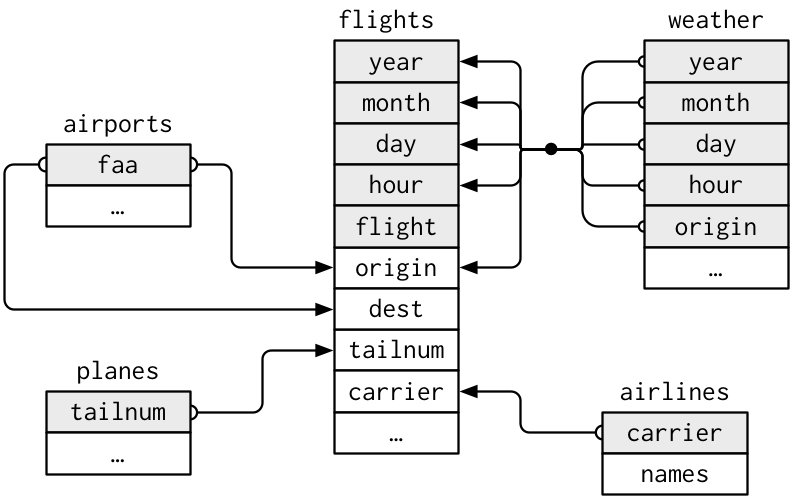
\includegraphics[width=0.7\linewidth,height=0.5\textheight]{week3_5} \end{center}
\end{frame}

\begin{frame}[fragile]{Matching ``key'' variable names}
\protect\hypertarget{matching-key-variable-names}{}
In both the \texttt{flights} and \texttt{airlines} data frames, the key
variable we want to join/merge/match the rows by has the same name:
\textbf{carrier}.

\begin{itemize}
\tightlist
\item
  Let's use the \texttt{inner\_join()} function to join the two data
  frames, where the rows will be matched by the variable carrier, and
  then compare the resulting data frames:
\end{itemize}

\tiny

\begin{Shaded}
\begin{Highlighting}[]
\NormalTok{flights\_joined }\OtherTok{\textless{}{-}}\NormalTok{ flights }\SpecialCharTok{\%\textgreater{}\%} 
  \FunctionTok{inner\_join}\NormalTok{(airlines, }\AttributeTok{by =} \StringTok{"carrier"}\NormalTok{)}
\CommentTok{\#View(flights)}
\CommentTok{\#View(flights\_joined)}
\end{Highlighting}
\end{Shaded}

\normalsize

Observe that the \texttt{flights} and \texttt{flights\_joined} data
frames are identical except that \texttt{flights\_joined} has an
additional variable name.
\end{frame}

\begin{frame}[fragile]{Matching ``key'' variable names}
\protect\hypertarget{matching-key-variable-names-1}{}
A visual representation of the \texttt{inner\_join()} is shown below

\begin{center}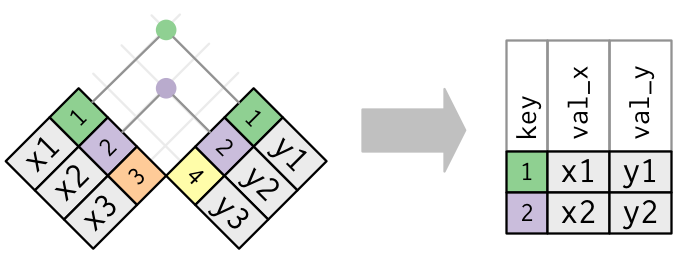
\includegraphics[width=0.6\linewidth,height=0.4\textheight]{week3_6} \end{center}

\begin{itemize}
\item
  There are other types of joins available,

  \begin{itemize}
  \tightlist
  \item
    such as left\_join(), right\_join(), outer\_join(), and
    anti\_join()),
  \item
    but the inner\_join() will solve nearly all of the problems you'll
    encounter in this class.
  \end{itemize}
\end{itemize}
\end{frame}

\begin{frame}[fragile]{Different ``key'' variable names}
\protect\hypertarget{different-key-variable-names}{}
\begin{itemize}
\item
  Say instead you are interested in the destinations of all domestic
  flights departing NYC in 2013,

  \begin{itemize}
  \tightlist
  \item
    and you ask yourself questions like: ``What cities are these
    airports in?'', or ``Is''ORD'' Orlando?'', or ``Where is''FLL''?''
  \end{itemize}
\item
  The \texttt{airports} data frame contains the airport codes for each
  airport:
\end{itemize}

\small

\begin{Shaded}
\begin{Highlighting}[]
\CommentTok{\#View(airports)}
\end{Highlighting}
\end{Shaded}

\normalsize

\begin{itemize}
\item
  However, if you look at both the \texttt{airports} and
  \texttt{flights} data frames, you'll find that the airport codes are
  in variables that have different names.

  \begin{itemize}
  \tightlist
  \item
    In \texttt{airports} the airport code is in \texttt{faa}.
  \item
    whereas in \texttt{flights} the destination airport codes are in
    \texttt{dest}.
  \item
    This fact is further highlighted in the visual representation of the
    relationships between these data frames.
  \end{itemize}
\end{itemize}
\end{frame}

\begin{frame}[fragile]{Different ``key'' variable names}
\protect\hypertarget{different-key-variable-names-1}{}
In order to join these two data frames by airport code, our
\texttt{inner\_join()} operation will use the
\texttt{by\ =\ c("dest"\ =\ "faa")} argument:

\small

\begin{Shaded}
\begin{Highlighting}[]
\NormalTok{flights\_with\_airport\_names }\OtherTok{\textless{}{-}}\NormalTok{ flights }\SpecialCharTok{\%\textgreater{}\%} 
  \FunctionTok{inner\_join}\NormalTok{(airports, }\AttributeTok{by =} \FunctionTok{c}\NormalTok{(}\StringTok{"dest"} \OtherTok{=} \StringTok{"faa"}\NormalTok{))}
\CommentTok{\#View(flights\_with\_airport\_names)}
\end{Highlighting}
\end{Shaded}

\normalsize
\end{frame}

\begin{frame}[fragile]{Different ``key'' variable names}
\protect\hypertarget{different-key-variable-names-2}{}
Let's construct the chain of pipe operators \texttt{\%\textgreater{}\%}
that computes the number of flights from NYC to each destination, but
also includes information about each destination airport:

\tiny

\begin{Shaded}
\begin{Highlighting}[]
\NormalTok{named\_dests }\OtherTok{\textless{}{-}}\NormalTok{ flights }\SpecialCharTok{\%\textgreater{}\%}
  \FunctionTok{group\_by}\NormalTok{(dest) }\SpecialCharTok{\%\textgreater{}\%}
  \FunctionTok{summarize}\NormalTok{(}\AttributeTok{num\_flights =} \FunctionTok{n}\NormalTok{()) }\SpecialCharTok{\%\textgreater{}\%}
  \FunctionTok{arrange}\NormalTok{(}\FunctionTok{desc}\NormalTok{(num\_flights)) }\SpecialCharTok{\%\textgreater{}\%}
  \FunctionTok{inner\_join}\NormalTok{(airports, }\AttributeTok{by =} \FunctionTok{c}\NormalTok{(}\StringTok{"dest"} \OtherTok{=} \StringTok{"faa"}\NormalTok{)) }\SpecialCharTok{\%\textgreater{}\%}
  \FunctionTok{rename}\NormalTok{(}\AttributeTok{airport\_name =}\NormalTok{ name)}
\NormalTok{named\_dests}
\end{Highlighting}
\end{Shaded}

\begin{verbatim}
## # A tibble: 101 x 9
##    dest  num_flights airport_name             lat    lon   alt    tz dst   tzone
##    <chr>       <int> <chr>                  <dbl>  <dbl> <dbl> <dbl> <chr> <chr>
##  1 ORD         17283 Chicago Ohare Intl      42.0  -87.9   668    -6 A     Amer~
##  2 ATL         17215 Hartsfield Jackson At~  33.6  -84.4  1026    -5 A     Amer~
##  3 LAX         16174 Los Angeles Intl        33.9 -118.    126    -8 A     Amer~
##  4 BOS         15508 General Edward Lawren~  42.4  -71.0    19    -5 A     Amer~
##  5 MCO         14082 Orlando Intl            28.4  -81.3    96    -5 A     Amer~
##  6 CLT         14064 Charlotte Douglas Intl  35.2  -80.9   748    -5 A     Amer~
##  7 SFO         13331 San Francisco Intl      37.6 -122.     13    -8 A     Amer~
##  8 FLL         12055 Fort Lauderdale Holly~  26.1  -80.2     9    -5 A     Amer~
##  9 MIA         11728 Miami Intl              25.8  -80.3     8    -5 A     Amer~
## 10 DCA          9705 Ronald Reagan Washing~  38.9  -77.0    15    -5 A     Amer~
## # i 91 more rows
\end{verbatim}

\normalsize
\end{frame}

\begin{frame}[fragile]{Multiple ``key'' variables}
\protect\hypertarget{multiple-key-variables}{}
\begin{itemize}
\item
  Say instead we want to join two data frames by multiple key variables.
\item
  For example, from the visual representation of the relationships
  between the data frame:

  \begin{itemize}
  \tightlist
  \item
    we see that in order to join the \texttt{flights} and
    \texttt{weather} data frames, we need more than one key variable:
    \texttt{year}, \texttt{month}, \texttt{day}, \texttt{hour}, and
    \texttt{origin}.
  \item
    This is because the combination of these 5 variables act to uniquely
    identify each observational unit in the weather data frame: hourly
    weather recordings at each of the 3 NYC airports.
  \end{itemize}
\item
  We achieve this by specifying a vector of key variables to join by
  using the \texttt{c()} function.

  \begin{itemize}
  \tightlist
  \item
    Recall, this function is is short for ``combine'' or
    ``concatenate.''
  \end{itemize}
\end{itemize}
\end{frame}

\begin{frame}[fragile]{Multiple ``key'' variables}
\protect\hypertarget{multiple-key-variables-1}{}
\tiny

\begin{Shaded}
\begin{Highlighting}[]
\NormalTok{flights\_weather\_joined }\OtherTok{\textless{}{-}}\NormalTok{ flights }\SpecialCharTok{\%\textgreater{}\%}
  \FunctionTok{inner\_join}\NormalTok{(weather, }\AttributeTok{by =} \FunctionTok{c}\NormalTok{(}\StringTok{"year"}\NormalTok{, }\StringTok{"month"}\NormalTok{, }\StringTok{"day"}\NormalTok{, }\StringTok{"hour"}\NormalTok{, }\StringTok{"origin"}\NormalTok{))}
\CommentTok{\#View(flights\_weather\_joined)}
\end{Highlighting}
\end{Shaded}

\normalsize
\end{frame}

\begin{frame}[fragile]{\texttt{select} variables}
\protect\hypertarget{select-variables}{}
\begin{center}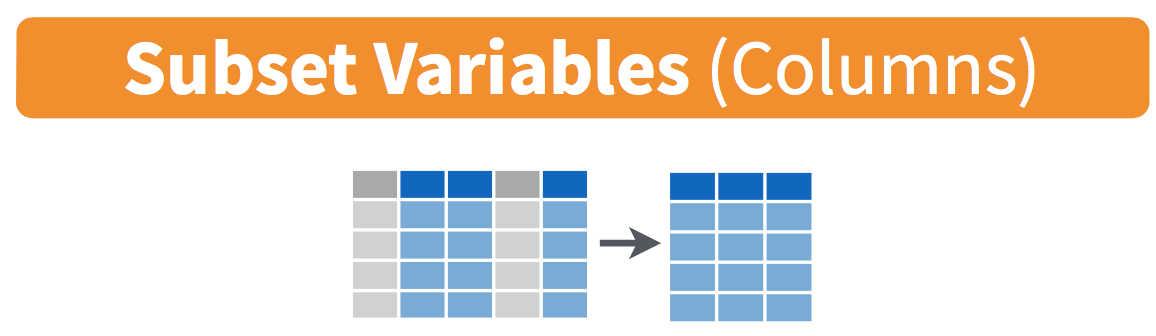
\includegraphics[width=0.7\linewidth,height=0.5\textheight]{week3_8} \end{center}

We've seen that the \texttt{flights} data frame in the
\texttt{nycflights13} package contains 19 different variables.

\tiny

\begin{Shaded}
\begin{Highlighting}[]
\CommentTok{\#glimpse(flights)}
\end{Highlighting}
\end{Shaded}

\normalsize
\end{frame}

\begin{frame}[fragile]{\texttt{select} variables}
\protect\hypertarget{select-variables-1}{}
However, say you only need two of these 19 variables, say
\texttt{carrier} and \texttt{flight}. You can \texttt{select()} these
two variables:

\tiny

\begin{Shaded}
\begin{Highlighting}[]
\NormalTok{flights\_sub }\OtherTok{\textless{}{-}}\NormalTok{flights }\SpecialCharTok{\%\textgreater{}\%} 
  \FunctionTok{select}\NormalTok{(carrier, flight)}
\end{Highlighting}
\end{Shaded}

\normalsize

Let's say instead you want to drop, or de-select, certain variables. For
example, lets say we want to remove the \texttt{year} in the
\texttt{flights} data frame. We can deselect year by using the
\texttt{-} sign:

\tiny

\begin{Shaded}
\begin{Highlighting}[]
\NormalTok{flights\_no\_year }\OtherTok{\textless{}{-}}\NormalTok{ flights }\SpecialCharTok{\%\textgreater{}\%} \FunctionTok{select}\NormalTok{(}\SpecialCharTok{{-}}\NormalTok{year)}
\end{Highlighting}
\end{Shaded}

\normalsize
\end{frame}

\begin{frame}[fragile]{\texttt{select} variables}
\protect\hypertarget{select-variables-2}{}
Another way of selecting columns/variables is by specifying a range of
columns:

\tiny

\begin{Shaded}
\begin{Highlighting}[]
\NormalTok{flight\_arr\_times }\OtherTok{\textless{}{-}}\NormalTok{ flights }\SpecialCharTok{\%\textgreater{}\%} \FunctionTok{select}\NormalTok{(month}\SpecialCharTok{:}\NormalTok{day, arr\_time}\SpecialCharTok{:}\NormalTok{sched\_arr\_time)}
\CommentTok{\#flight\_arr\_times}
\end{Highlighting}
\end{Shaded}

\normalsize

This will \texttt{select()} all columns between \texttt{month} and
\texttt{day}, as well as between \texttt{arr\_time} and
\texttt{sched\_arr\_time}, and drop the rest.
\end{frame}

\begin{frame}[fragile]{\texttt{select} variables}
\protect\hypertarget{select-variables-3}{}
The \texttt{select()} function can also be used to reorder columns when
used with the \texttt{everything()} helper function.

\begin{itemize}
\item
  For example, suppose we want the \texttt{hour}, \texttt{minute}, and
  \texttt{time\_hour} variables to appear immediately after the
  \texttt{year}, \texttt{month}, and \texttt{day} variables, while not
  discarding the rest of the variables.
\item
  In the following code, \texttt{everything()} will pick up all
  remaining variables:
\end{itemize}

\tiny

\begin{Shaded}
\begin{Highlighting}[]
\NormalTok{flights\_reorder }\OtherTok{\textless{}{-}}\NormalTok{ flights }\SpecialCharTok{\%\textgreater{}\%} 
  \FunctionTok{select}\NormalTok{(year, month, day, hour, minute, time\_hour, }\FunctionTok{everything}\NormalTok{())}
\CommentTok{\#glimpse(flights\_reorder)}
\end{Highlighting}
\end{Shaded}

\normalsize
\end{frame}

\begin{frame}[fragile]{\texttt{select} variables}
\protect\hypertarget{select-variables-4}{}
Lastly, the helper functions \texttt{starts\_with()},
\texttt{ends\_with()}, and \texttt{contains(}) can be used to select
variables/columns that match those conditions. As examples,

\tiny

\begin{Shaded}
\begin{Highlighting}[]
\NormalTok{flights\_sub1}\OtherTok{\textless{}{-}}\NormalTok{flights }\SpecialCharTok{\%\textgreater{}\%} \FunctionTok{select}\NormalTok{(}\FunctionTok{starts\_with}\NormalTok{(}\StringTok{"a"}\NormalTok{))}
\NormalTok{flights\_sub2}\OtherTok{\textless{}{-}}\NormalTok{flights }\SpecialCharTok{\%\textgreater{}\%} \FunctionTok{select}\NormalTok{(}\FunctionTok{ends\_with}\NormalTok{(}\StringTok{"delay"}\NormalTok{))}
\NormalTok{flights\_sub3}\OtherTok{\textless{}{-}}\NormalTok{flights }\SpecialCharTok{\%\textgreater{}\%} \FunctionTok{select}\NormalTok{(}\FunctionTok{contains}\NormalTok{(}\StringTok{"time"}\NormalTok{))}
\end{Highlighting}
\end{Shaded}

\normalsize
\end{frame}

\begin{frame}{Summary table}
\protect\hypertarget{summary-table}{}
\begin{center}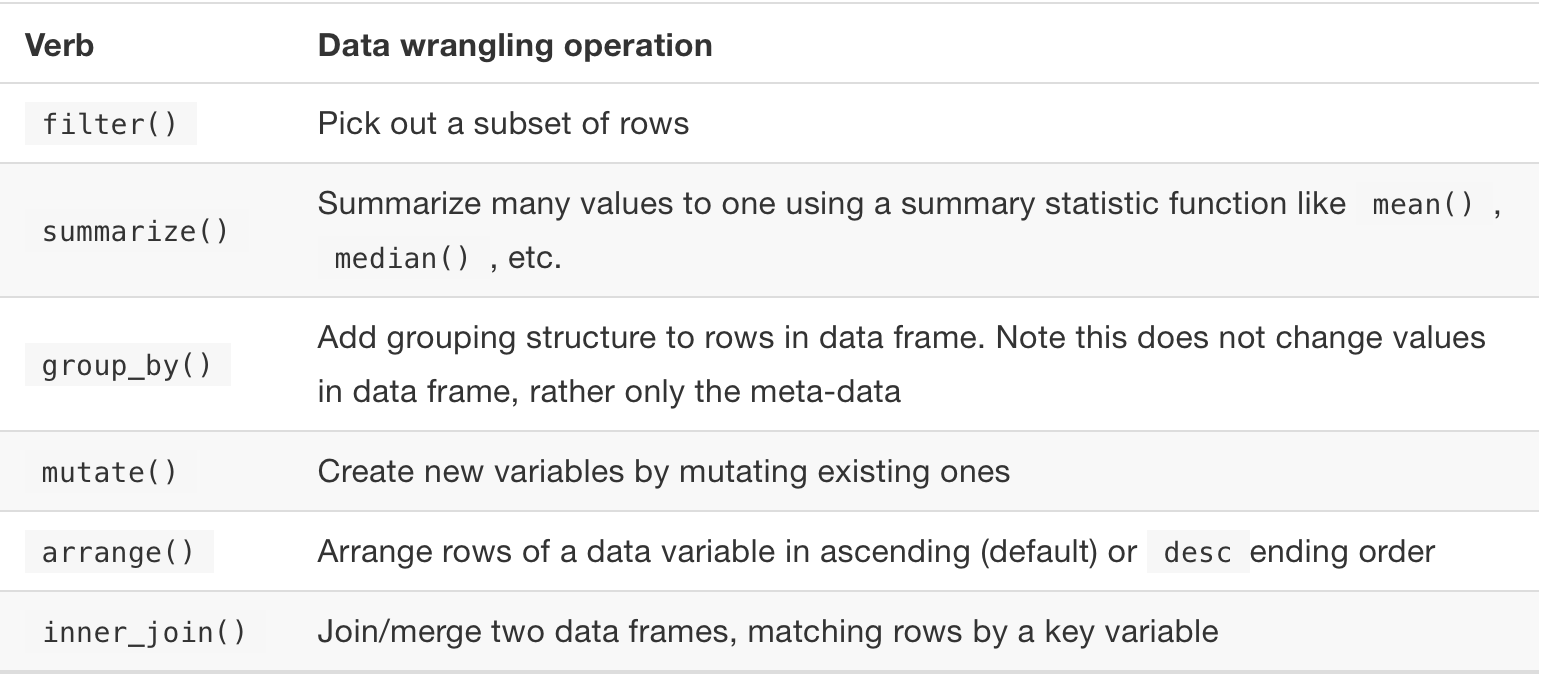
\includegraphics[width=0.8\linewidth,height=0.6\textheight]{week3_7} \end{center}
\end{frame}

\hypertarget{tidy-data}{%
\section{``Tidy'' data}\label{tidy-data}}

\begin{frame}[fragile]{``Tidy'' data}
\protect\hypertarget{tidy-data-1}{}
Let's now learn about the concept of \textbf{``tidy''} data format.

\begin{itemize}
\tightlist
\item
  We focus on the \texttt{drinks} data frame in the
  \texttt{fivethirtyeight} package.
\end{itemize}

\tiny

\begin{Shaded}
\begin{Highlighting}[]
\FunctionTok{library}\NormalTok{(fivethirtyeight)}
\NormalTok{drinks\_smaller }\OtherTok{\textless{}{-}}\NormalTok{ drinks }\SpecialCharTok{\%\textgreater{}\%} 
  \FunctionTok{filter}\NormalTok{(country }\SpecialCharTok{\%in\%} \FunctionTok{c}\NormalTok{(}\StringTok{"USA"}\NormalTok{, }\StringTok{"China"}\NormalTok{, }\StringTok{"Italy"}\NormalTok{, }\StringTok{"Saudi Arabia"}\NormalTok{)) }\SpecialCharTok{\%\textgreater{}\%} 
  \FunctionTok{select}\NormalTok{(}\SpecialCharTok{{-}}\NormalTok{total\_litres\_of\_pure\_alcohol) }\SpecialCharTok{\%\textgreater{}\%} 
  \FunctionTok{rename}\NormalTok{(}\AttributeTok{beer =}\NormalTok{ beer\_servings, }\AttributeTok{spirit =}\NormalTok{ spirit\_servings, }\AttributeTok{wine =}\NormalTok{ wine\_servings)}
\NormalTok{drinks\_smaller}
\end{Highlighting}
\end{Shaded}

\begin{verbatim}
## # A tibble: 4 x 4
##   country       beer spirit  wine
##   <chr>        <int>  <int> <int>
## 1 China           79    192     8
## 2 Italy           85     42   237
## 3 Saudi Arabia     0      5     0
## 4 USA            249    158    84
\end{verbatim}

\normalsize
\end{frame}

\begin{frame}[fragile]{``Tidy'' data}
\protect\hypertarget{tidy-data-2}{}
The \texttt{drinks\_smaller} data frame, cannot be used to create the
side-by-side barplot show below.

\small

\begin{center}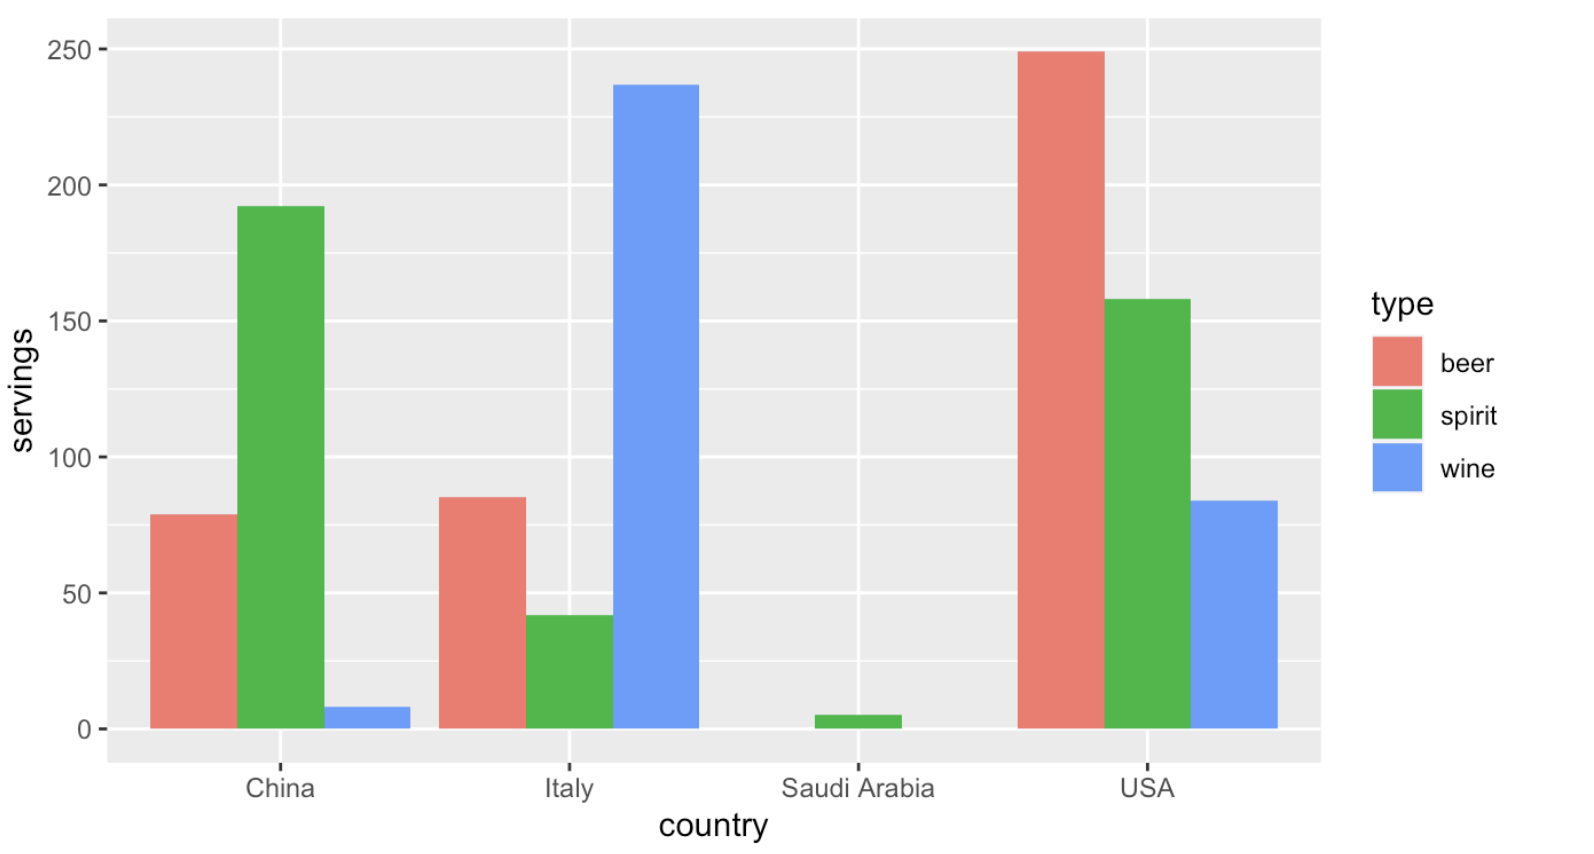
\includegraphics[width=0.7\linewidth,height=0.5\textheight]{week3new1} \end{center}
\normalsize

why?
\end{frame}

\begin{frame}{``Tidy'' data}
\protect\hypertarget{tidy-data-3}{}
\begin{itemize}
\item
  Let's break down the grammar of graphics we introduced earlier:

  \begin{itemize}
  \item
    The categorical variable country with four levels (China, Italy,
    Saudi Arabia, USA) would have to be mapped to the x-position of the
    bars.
  \item
    The numerical variable servings would have to be mapped to the
    y-position of the bars (the height of the bars).
  \item
    The categorical variable type with three levels (beer, spirit, wine)
    would have to be mapped to the fill color of the bars.
  \end{itemize}
\item
  To recreate the barplot above, our data frame should be in the
  \textbf{``tidy''} format.
\end{itemize}
\end{frame}

\begin{frame}{``Tidy'' data: Definition}
\protect\hypertarget{tidy-data-definition}{}
The word ``tidy'' in data science means that your data follows a
standardized format.

\begin{itemize}
\item
  ``Tidy'' data is a standard way of mapping the meaning of a dataset to
  its structure. A dataset is messy or tidy depending on how rows,
  columns and tables are matched up with observations, variables and
  types.
\item
  In tidy data:

  \begin{itemize}
  \tightlist
  \item
    Each variable forms a column.
  \item
    Each observation forms a row.
  \item
    Each type of observational unit forms a table.
  \end{itemize}
\end{itemize}

\small

\begin{center}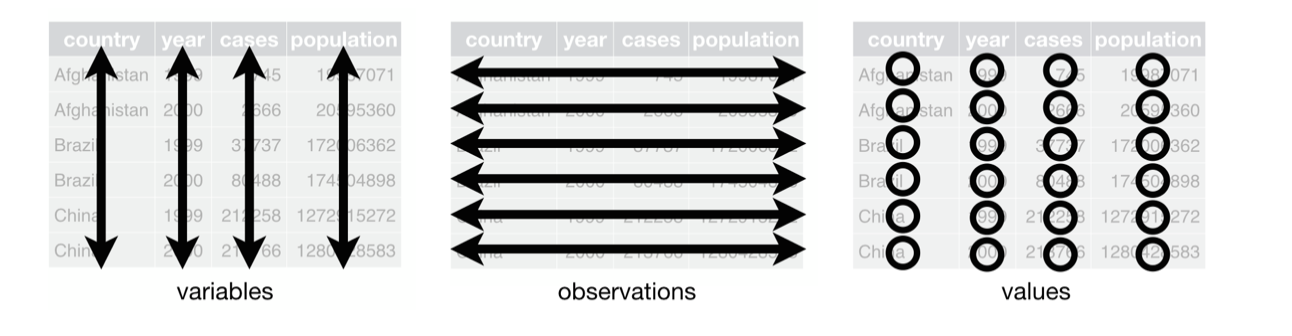
\includegraphics[width=0.6\linewidth,height=0.25\textheight]{week3new2} \end{center}
\normalsize
\end{frame}

\begin{frame}{``Tidy'' data: Definition}
\protect\hypertarget{tidy-data-definition-1}{}
Stock prices (non-tidy format): \small

\begin{center}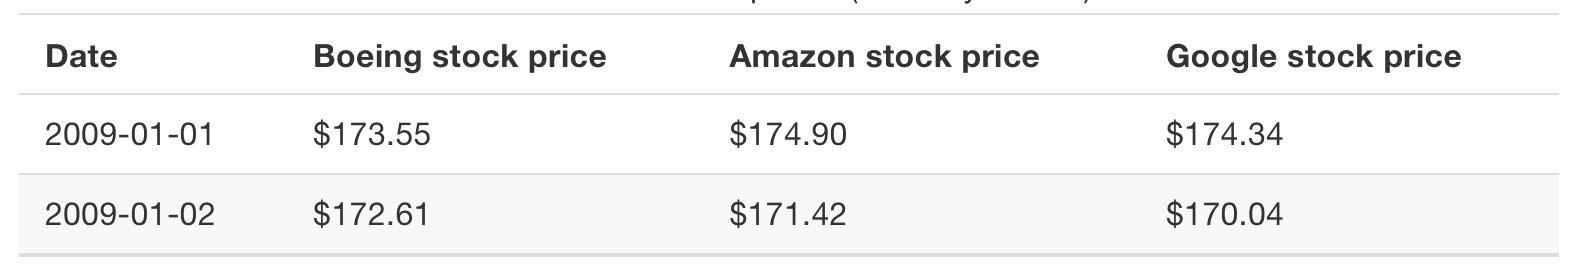
\includegraphics[width=0.7\linewidth,height=0.25\textheight]{week3new3} \end{center}
\normalsize

Stock prices (tidy format):

\small

\begin{center}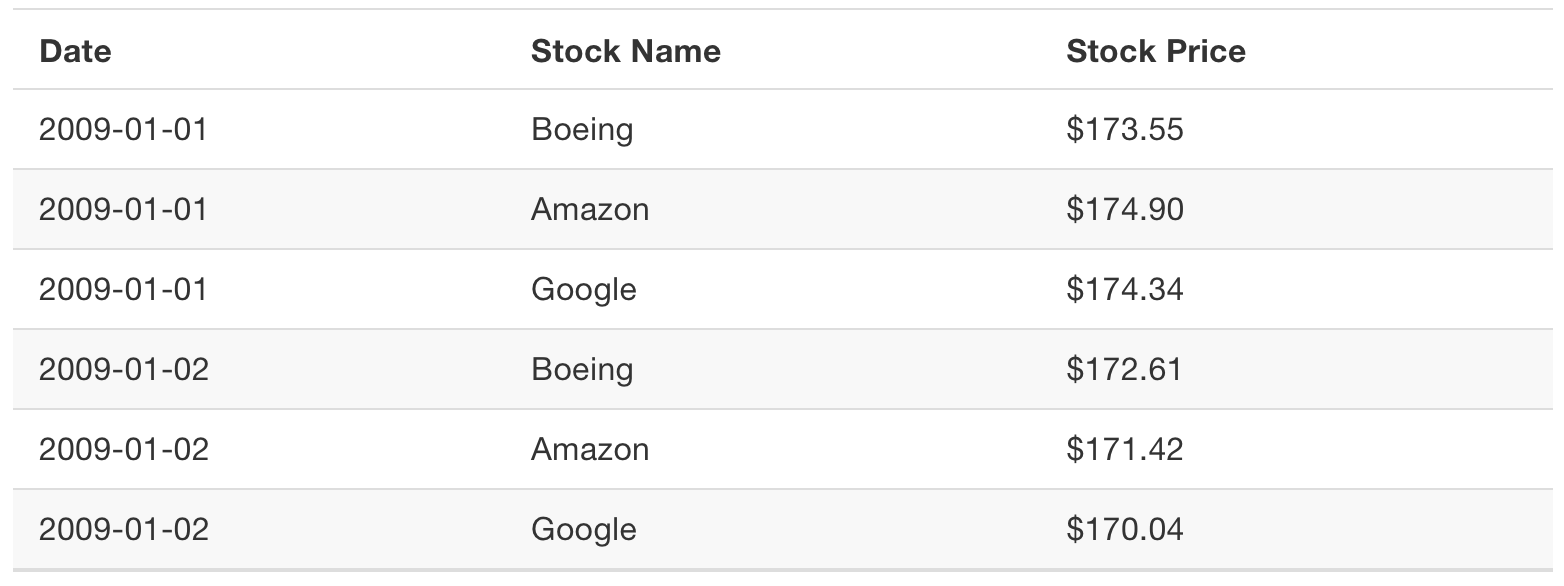
\includegraphics[width=0.6\linewidth,height=0.4\textheight]{week3new4} \end{center}
\normalsize
\end{frame}

\begin{frame}{``Tidy'' data: Definition}
\protect\hypertarget{tidy-data-definition-2}{}
\begin{itemize}
\item
  Observe that:

  \begin{itemize}
  \tightlist
  \item
    The non-tidy format of the stock prices is what's known as ``wide''
    format, whereas - the tidy format is known as ``long/narrow''
    format.
  \end{itemize}
\item
  In the context of doing data science, \textbf{long/narrow} format is
  also known as \textbf{``tidy''} format.
\item
  In order to use the ggplot2 and dplyr packages for data visualization
  and data wrangling, your input data frames must be in ``tidy'' format.
\item
  Thus, all non-``tidy'' data must be converted to ``tidy'' format
  first.
\end{itemize}
\end{frame}

\begin{frame}[fragile]{Coverting to ``Tidy'' format}
\protect\hypertarget{coverting-to-tidy-format}{}
We convert the \texttt{drinks\_smaller} data to ``tidy'' format by using
the \texttt{pivot\_longer()} function from the \texttt{tidyr} package:

\tiny

\begin{Shaded}
\begin{Highlighting}[]
\FunctionTok{library}\NormalTok{(tidyr)}
\NormalTok{drinks\_smaller\_tidy }\OtherTok{\textless{}{-}}\NormalTok{ drinks\_smaller }\SpecialCharTok{\%\textgreater{}\%} 
  \FunctionTok{pivot\_longer}\NormalTok{(}\AttributeTok{names\_to =} \StringTok{"type"}\NormalTok{, }
               \AttributeTok{values\_to =} \StringTok{"servings"}\NormalTok{, }
               \AttributeTok{cols =} \SpecialCharTok{{-}}\NormalTok{country)}
\NormalTok{drinks\_smaller\_tidy}
\end{Highlighting}
\end{Shaded}

\begin{verbatim}
## # A tibble: 12 x 3
##    country      type   servings
##    <chr>        <chr>     <int>
##  1 China        beer         79
##  2 China        spirit      192
##  3 China        wine          8
##  4 Italy        beer         85
##  5 Italy        spirit       42
##  6 Italy        wine        237
##  7 Saudi Arabia beer          0
##  8 Saudi Arabia spirit        5
##  9 Saudi Arabia wine          0
## 10 USA          beer        249
## 11 USA          spirit      158
## 12 USA          wine         84
\end{verbatim}

\normalsize
\end{frame}

\begin{frame}[fragile]{Coverting to ``Tidy'' format}
\protect\hypertarget{coverting-to-tidy-format-1}{}
These will produce same results \tiny

\begin{Shaded}
\begin{Highlighting}[]
\FunctionTok{library}\NormalTok{(tidyr)}
\NormalTok{drinks\_smaller }\SpecialCharTok{\%\textgreater{}\%} 
  \FunctionTok{pivot\_longer}\NormalTok{(}\AttributeTok{names\_to =} \StringTok{"type"}\NormalTok{, }
               \AttributeTok{values\_to =} \StringTok{"servings"}\NormalTok{, }
               \AttributeTok{cols =} \FunctionTok{c}\NormalTok{(beer, spirit, wine))}


\NormalTok{drinks\_smaller }\SpecialCharTok{\%\textgreater{}\%} 
  \FunctionTok{pivot\_longer}\NormalTok{(}\AttributeTok{names\_to =} \StringTok{"type"}\NormalTok{, }
               \AttributeTok{values\_to =} \StringTok{"servings"}\NormalTok{, }
               \AttributeTok{cols =}\NormalTok{ beer}\SpecialCharTok{:}\NormalTok{wine)}
\end{Highlighting}
\end{Shaded}

\normalsize
\end{frame}

\begin{frame}[fragile]{Coverting to ``Tidy'' format}
\protect\hypertarget{coverting-to-tidy-format-2}{}
\tiny

\begin{Shaded}
\begin{Highlighting}[]
\FunctionTok{library}\NormalTok{(tidyr)}
\FunctionTok{ggplot}\NormalTok{(drinks\_smaller\_tidy, }\FunctionTok{aes}\NormalTok{(}\AttributeTok{x =}\NormalTok{ country, }\AttributeTok{y =}\NormalTok{ servings, }\AttributeTok{fill =}\NormalTok{ type)) }\SpecialCharTok{+}
  \FunctionTok{geom\_col}\NormalTok{(}\AttributeTok{position =} \StringTok{"dodge"}\NormalTok{)}
\end{Highlighting}
\end{Shaded}

\begin{center}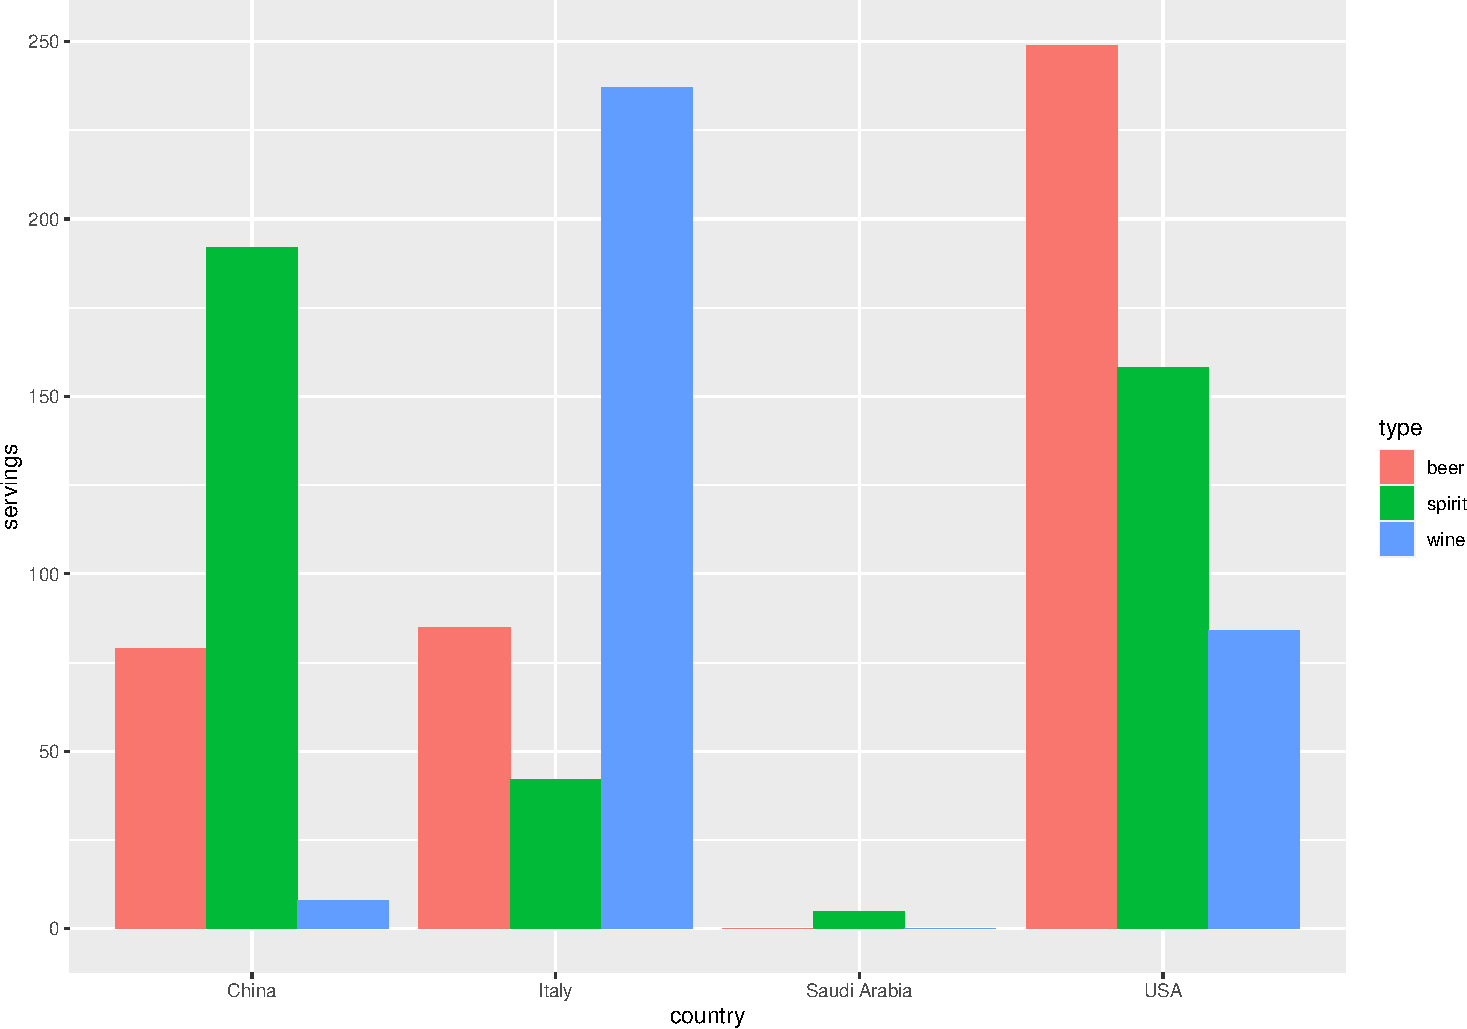
\includegraphics[width=0.8\linewidth,height=0.5\textheight]{Week3_files/figure-beamer/unnamed-chunk-52-1} \end{center}
\normalsize
\end{frame}

\end{document}
